% vim: set textwidth=78 autoindent:

\section{Integrazione con GRASS GIS}\label{sec:grass}\index{GRASS}

% when the revision of a section has been finalized, 
% comment out the following line:
%\updatedisclaimer

Il plugin GRASS consente l'accesso ai dati e alle funzioni di GRASS
GIS~\cite{GRASSweb}, inclusa la visualizzazione di strati raster e vettoriali,
la digitalizzazione di strati vettoriali, la modifica degli attributi e la
creazione di nuovi vettori, e l'analisi di dati GRASS 2D e 3D tramite più di
300 moduli GRASS.

In questa Sezione verranno forniti un'introduzione sulle funzionalità del plugin
e qualche esempio sulla gestione e l'utilizzo di dati GRASS. Quando viene
abilitato il plugin GRASS coem descritto alla Sezione~\ref{sec:starting_grass},
nella barra sono disponibili i seguenti strumenti:
 
\begin{itemize}
\item \toolbtntwo{grass_open_mapset}{Apri mapset}
\item \toolbtntwo{grass_new_mapset}{Nuovo mapset}
\item \toolbtntwo{grass_close_mapset}{Chiudi mapset}
\item \toolbtntwo{grass_add_vector}{Aggiungi vettoriale GRASS}
\item \toolbtntwo{grass_add_raster}{Aggiungi raster GRASS}
\item \toolbtntwo{grass_new_vector_layer}{Crea nuovo vettoriale GRASS}
\item \toolbtntwo{grass_edit}{Modifica vettoriale GRASS}
\item \toolbtntwo{grass_tools}{Apri strumenti GRASS}
%\item \toolbtntwo{grass_shell}{Open GRASS Shell}
\item \toolbtntwo{grass_region}{Visualizza GRASS regione attuale} 
\item \toolbtntwo{grass_region_edit}{Modifica region GRASS attuale}
\end{itemize}

\subsection{Avviare il plugin GRASS}\label{sec:starting_grass}
\index{GRASS!starting QGIS}

Per usare le funzioni GRASS e/o visualizzare livelli raster e vettoriali in
formato GRASS in QGIS, bisogna selezionare e caricare il plugin GRASS con il
Gestore plugin. 
Cliccare quindi sul menù \mainmenuopt{Plugins} > \mainmenuopt{Gestione plugins}, 
selezionare \dropmenuopt{GRASS} e cliccare \button{OK}. 

Ora è quindi possibile caricare livelli raster e vettoriali da una \filename{LOCATION}
GRASS esistente (si veda la Sezione \ref{sec:load_grassdata}). È anche
possibile creare una nuova \filename{LOCATION} GRASS in QGIS (si veda la
Sezione \ref{sec:create_loc}) e importare in essa dati raster e vettoriali (si
veda la Sezione \ref{sec:import_loc_data}) per ulteriori analisi con gli
strumenti GRASS (si veda la Sezione \ref{subsec:grass_toolbox}).

\subsection{Caricare livelli raster e vettoriali GRASS}\label{sec:load_grassdata}\index{GRASS!loading data}

Con il plugin GRASS, possono essere caricati layer raster o vettoriali
usando il pulsante appropriato nella barra strumenti. Come esempio si
consideri il set di dati Alaska (si veda la Sezione \ref{label_sampledata}).
Esso include un piccola \filename{LOCATION} GRASS campione contenente 3 layers
vettoriali e una mappa di altitudine raster.

\begin{enumerate}
  \item Creare una nuova cartella \filename{grassdata}, nella quale scaricare
  il set di dati Alaska denominato \filename{qgis\_sample\_data.zip}
  dall'indirizzo web \url{http://download.osgeo.org/qgis/data/} e decomprimere
  il file nella cartella \filename{grassdata}. 
  \item Avviare QGIS.
  \item Se non è già stato fatto in precedenti sessioni di QGIS, caricare il
  plugin GRASS cliccando su\mainmenuopt{Plugins} > \mainmenuopt{Gestione
  plugins} e selzionare \dropmenuopt{GRASS}. La barra GRASS apparirà nella
  barra strumenti.
  \item Nella barra strumenti GRASS, cliccare sull'icona
  \toolbtntwo{grass_open_mapset}{Apri mapset} per aprire la finestra
  \filename{Seleziona Mapset}.
  \item Alla voce \filename{Gisdbase} inserire l'indirizzo completo o navigare
  fino alla cartella \filename{grassdata} appena creata.
  \item Dovrebbe ora essere possibile selezionare la \filename{LOCATION
  alaska} e il MAPSET \filename{demo}. 
  \item Cliccare su \button{OK}. Si noti che ora alcuni degli strumenti
  precedentemente disabilitati sono divenuti attivi.
  \item Cliccare su \toolbtntwo{grass_add_raster}{Aggiungi raster GRASS},
  scegliere la mappa denominata \filename{gtopo30} e cliccare su \button{OK}.
  Verrà visualizzato il layer delle elevazioni del terreno.
  \item Cliccare su \toolbtntwo{grass_add_vector}{Aggiungi vettoriale GRASS},
  selezionare la mappa denominata \filename{alaska} e cliccare su \button{OK}.
  Il confine dell'Alaska verrà sovrapposto alla mappa gtopo30 map. Ora è
  possibile adattare le proprietà del layer come descrittto al capitolo
  \ref{sec:vectorprops}, ovvero cambiare la trasparenza, il colore di
  riempimento e del contorno dell'elemento.
  \item Caricare anche gli altri due layer vettoriali denominati
  \filename{rivers} e \filename{airports} e modificarne le proprietà.
\end{enumerate}

Come dimostrato è quindi molto semplice caricare dati raster e vettoriali in
formato GRASS in QGIS. Si veda la sezione seguente per sapere come editare
dati GRASS e creare nuove \filename{LOCATION}. Ulteriori \filename{LOCATIONs}
campione di GRASS sono disponibili sul siti di GRASS all'indirizzo
\url{http://grass.osgeo.org/download/data.php}.

\begin{Tip}\caption{\textsc{Caricare dati GRASS}}
\qgistip{Se si presentano problemi nel caricare dati o QGIS termina
inaspettatamente, assicurarsi di aver caricato il plugin GRASS correttamente
come descritto alla Sezione \ref{sec:starting_grass}.
}
\end{Tip} 

\subsection{LOCATION e MAPSET in GRASS}\label{sec:about_loc}

GRASS organizza i propri in cartelle alle quali si fa riferimento con la
denominazione GISDBASE. Queste cartelle, spesso chiamate \filename{grassdata},
devono essere create prima di iniziare a lavorare con il plugin GRASS in QGIS.
In queste directori, i dati GRASS sono organizzati per progetti inseriti in
sottocartelle chiamate \filename{LOCATION}. 
Ogni \filename{LOCATION} è definita da un sistema di coordinate, da un sistema
di proiezione e dall'estensione geografica. La \filename{LOCATION} può avere a
sua volta molte sottocartelle \filename{MAPSETs} usate per suddividere il
progetto in diversi argomenti, sottoregioni o spazi di lavoro per i diversi
membri del team che vi sta lavorando (Neteler \& Mitasova 2008
\cite{neteler_mitasova08}). Per analizzare layers raster e vettoriali con i
moduli GRASS, bisogna importarli in una \filename{LOCATION} GRASS.
\footnote{Questo non è proprio vero - con i moduli GRASS \filename{r.external}
e \filename{v.external} è possibile creare collegamenti in sola lettura ai
dati GDAL/OGR supportati senza che sia necessario effettuare l'importazione.
Tuttavia siccome questa non è la modalità predefinita per i principianti
questa funzione non verrà descritta.}

\begin{figure}[ht]
\begin{center}
\caption{Organizzazzione dei dati GRASS nella LOCATION campione alaska
(adattato da from Neteler \& Mitasova 2008 \cite{neteler_mitasova08})}\label{fig:grass_location}\smallskip

\includegraphics[clip=true]{grass_location}
\end{center}  
\end{figure}

\subsubsection{Creare una nuova LOCATION GRASS}\label{sec:create_loc}

Per questo e per tutti i successivi esempi riguardanti GRASS GIS verrà usata la \filename{LOCATION
alaska} campione, che è proiettata nel sistema Albers Equal Area con unità di
misura in metri, creata dal set di dati campione di QGIS. Sarà utile scaricare
ed installare il set di dati sul proprio computer \ref{label_sampledata}).

\begin{figure}[ht]
\begin{center}
\caption{Creazione di una nuova LOCATION GRASS o di un nuovo MAPSET in QGIS \nixcaption}
\label{fig:create_grass_location}\smallskip
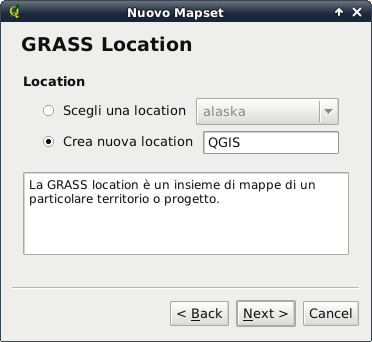
\includegraphics[clip=true, width=10cm]{create_grass_location}
\end{center}  
\end{figure}

\begin{enumerate}
  \item Avviare QGIS e assicurarsi che il plugin GRASS sia caricato
  \item Visualizzare lo shapefile \filename{alaska.shp} (si veda la Sezione
  \ref{sec:load_shapefile}) dal set di dati alaska~\ref{label_sampledata}.
  \item Nella barra strumenti GRASS, cliccare sull'icona
  \toolbtntwo{grass_new_mapset}{Nuovo mapset} per avviare la procedura guidata.
  \item Selezionare la cartella contenente il database GRASS (GISDBASE)
  denominata \filename{grassdata} o crearne una nuova in cui ospitare la nuova
  \filename{LOCATION} usando il gestore di file installato sul proprio
  computer. Cliccare su \button{Next}. 
  \item Per creare un nuovo \filename{MAPSET} in una \filename{LOCATION}
  esistente (si veda la Sezione~\ref{sec:add_mapset}) o per creare una nuova
  \filename{LOCATION}, selezionare l'opzione \radiobuttonon{Crea nuova
  location} (si veda la Figura \ref{fig:create_grass_location}).
  \item Inserire il nome della \filename{LOCATION} - nell'esempio abbiamo
  usato alaska, e cliccare su \button{Next} 
  \item Definire la proiezione cliccando sull'opzione
  \radiobuttonon{Proiezione} per abilitare l'elenco delle proiezioni 
  % Notare che il codice 5000 non è coretto. Attendere allineamento upstream
  \item Scegliere la proiezione Albers Equal Area Alaska (metri). Siccome ne
  conosciamo l'identificativo EPSG che è 5000, inserirlo nella casella di
  ricerca. (Nota: se si vuole ripetere il processo per un'altra
  \filename{LOCATION} e non si è memorizzato l'identificativo EPSG della
  proiezione, cliccare sull'icona   \toolbtntwo{mIconProjectionEnabled}{Stato CRS}
  nella parte destra inferiore della barra di stato (si veda la sezione \ref{label_projstart})).
  \item Cliccare su \button{Trova} per selezionare la proiezione
  \item Cliccare su \button{Next} 
  \item Per definire l'estensione della regione di default, bisonga inserire i
  limiti della \filename{LOCATION} verso nord, sud, est e ovest. Nel nostro
  esempio cliccare semplicemente sul pulsante \button{Imposta estensione
  attuale di QGIS}, per applicare l'estensione del layer caricato
  \filename{alaska.shp} come estensione di default della region GRASS.
  \item Cliccare su \button{Next} 
  \item Abbiamo anche bisogno di definire un \filename{MAPSET} interno alla
  location \filename{LOCATION}. Il nome è a scelta, nell'esempio abbiamo
  usato demo.
  \footnote{Quando si crea una nuova \filename{LOCATION}, GRASS crea
  automaticamente un \filename{MAPSET} speciale chiamato \filename{PERMANENT}
  designato a contenere i dati di base del progetto, l'estensione spaziale di
  default e la definizione del sistema di coordinate (Neteler \& Mitasova 2008 
  \cite{neteler_mitasova08}).}
  \item Controllare il riassunto per assicurarsi che le impostazioni siano
  corrette e cliccare su \button{Finish} 
  \item La nuova \filename{LOCATION alaska} e i \filename{MAPSETs demo}
  e \filename{PERMANENT} vengono creati. Il set di lavoro impostato per il
  lavoro corrente è il \filename{MAPSET demo}.
  \item Si noti che alcuni strumenti della barra di GRASS precedentemente
  disabilitati sono ora attivi.
\end{enumerate}

Per quanto possa essere apparsa lunga, questa procedura costitiusce un modo
veloce per creare una \filename{LOCATION}. La \filename{LOCATION alaska} è ora
pronta per l'importazione dei dati (si veda la Sezione \ref{sec:import_loc_data}).
È anche possibile usare dati raster e vettoriali esistenti nella
\filename{LOCATION alaska} campione in formato GRASS inclusi nel dataset
alaska di QGIS \ref{label_sampledata} e procedere alla Sezione \ref{label_vectmodel}.

\subsubsection{Aggiungere un nuovo MAPSET}\label{sec:add_mapset}

A user has only write access to a GRASS \filename{MAPSET} he created. This 
means, besides access to his own \filename{MAPSET}, each user can also read 
maps in other user's \filename{MAPSETs}, but he can modify or remove only 
the maps in his own \filename{MAPSET}. All \filename{MAPSETs} include a 
\filename{WIND} file that stores the current boundary coordinate values and 
the currently selected raster resolution (Neteler \& Mitasova 2008 
\cite{neteler_mitasova08}, see Section \ref{sec:grass_region}). 

\begin{enumerate}
  \item Start QGIS and make sure the GRASS plugin is loaded
  \item In the GRASS toolbar, click on the 
  \toolbtntwo{grass_open_mapset}{Apri mapset} icon to bring up the 
  \filename{MAPSET} wizard.
  \item Select the GRASS database (GISDBASE) folder \filename{grassdata} 
  with the \filename{LOCATION alaska}, where we want to add a further 
  \filename{MAPSET}, called test.
  \item Click \button{Next}. 
  \item We can use this wizard to create a new \filename{MAPSET} within an 
  existing \filename{LOCATION} or to create a new \filename{LOCATION} 
  altogether. Click on the radio button \radiobuttonon{Select location} 
  (see Figure \ref{fig:create_grass_location}) and click \button{Next}.
  \item Enter the name \filename{text} for the new \filename{MAPSET}. Below 
  in the wizard you see a list of existing \filename{MAPSETs} and its owners.
  \item Click \button{Next}, check out the summary to make sure it's all 
  correct and click \button{Finish} 
\end{enumerate}

\subsection{Importing data into a GRASS LOCATION}\label{sec:import_loc_data}

This Section gives an example how to import raster and vector data into the 
\filename{alaska} GRASS \filename{LOCATION} provided by the QGIS alaska 
dataset. Therefore we use a landcover raster map \filename{landcover.tif} 
and a vector polygone Shape \filename{lakes.shp} from the QGIS alaska 
dataset \ref{label_sampledata}.

\begin{enumerate}
  \item Start QGIS and make sure the GRASS plugin is loaded.
  \item In the GRASS toolbar, click the \toolbtntwo{grass_open_mapset}{Open 
  MAPSET} icon to bring up the \filename{MAPSET} wizard.
  \item Select as GRASS database the folder \filename{grassdata} in the QGIS 
  alaska dataset, as \filename{LOCATION alaska}, as \filename{MAPSET} 
  \filename{demo} and click \button{OK}.
  \item Now click the \toolbtntwo{grass_tools}{Apri strumenti GRASS} icon. The 
  GRASS Toolbox (see Section \ref{subsec:grass_toolbox}) dialog appears.
  \item To import the raster map \filename{landcover.tif}, click the module 
  \filename{r.in.gdal} in the \tab{Modules Tree} tab. This GRASS module 
  allows to import GDAL supported raster files into a GRASS 
  \filename{LOCATION}. The module dialog for \filename{r.in.gdal} appears.
  \item Browse to the folder \filename{raster} in the QGIS alaska dataset 
  and select the file \filename{landcover.tif}.
  \item As raster output name define \filename{landcover\_grass} and click 
  \button{Run}. In the \tab{Output} tab you see the currently running GRASS 
  command \filename{r.in.gdal -o input=/path/to/landcover.tif 
  output=landcover\_grass}.
  \item When it says \textbf{Succesfully finished} click \button{View output}. 
  The \filename{landcover\_grass} raster layer is now imported into GRASS and 
  will be visualized in the QGIS canvas.
  \item To import the vector shape \filename{lakes.shp}, click the module 
  \filename{v.in.ogr} in the \tab{Modules Tree} tab. This GRASS module allows 
  to import OGR supported vector files into a GRASS \filename{LOCATION}. The 
  module dialog for \filename{v.in.ogr} appears.
  \item Browse to the folder \filename{vmap0\_shapefiles} in the QGIS alaska 
  dataset and select the file \filename{lakes.shp} as OGR file.
  \item As vector output name define \filename{lakes\_grass} and click 
  \button{Run}. You don't have to care about the other options in this 
  example. In the \tab{Output} tab you see the currently running GRASS 
  command \filename{v.in.ogr -o dsn=/path/to/lakes.shp output=lakes\_grass}.
  \item When it says \textbf{Succesfully finished} click \button{View output}. 
  The \filename{lakes\_grass} vector layer is now imported into GRASS and will 
  be visualized in the QGIS canvas. 
\end{enumerate}


\subsection{The GRASS vector data model}\label{label_vectmodel}\index{GRASS!vector data
model}

It is important to understand the GRASS vector data model prior to
digitizing.\index{GRASS!digitizing} In general, GRASS uses a topological
vector model.\index{GRASS!topology} This means that areas are not represented
as closed polygons, but by one or more boundaries. A boundary between two
adjacent areas is digitized only once, and it is shared by both areas.
Boundaries must be connected without gaps. An area is identified (labeled) 
by the centroid of the area.

Besides boundaries and centroids, a vector map can also contain
points and lines. All these geometry elements can be mixed
in one vector and will be represented in different so called 'layers' inside
one GRASS vector map. So in GRASS a layer is not a vector or raster map but a
level inside a vector layer. This is important to distinguish carefully.
\footnote{Although it
is possible to mix geometry elements, it is unusual and even in GRASS only
used in special cases such as vector network analysis. Normally you should
prefere to store different geometry elements in different layers.}

It is possible to store more 'layers' in one vector dataset. For example,
fields, forests and lakes can be stored in one vector. Adjacent
forest and lake can share the same boundary, but they have separate attribute
tables. It is also possible to attach attributes to boundaries. For example,
the boundary between lake and forest is a road, so it can have a different 
attribute table.
 
The 'layer' of the feature is defined by 'layer' inside GRASS. 'Layer' is the 
number which defines if there are more than one layer inside the dataset, e.g. 
if the geometry is forest or lake. For now, it can be only a number, in the 
future GRASS will also support names as fields in the user interface.

Attributes can be stored inside the GRASS \filename{LOCATION} as DBase or 
SQLITE3 or in external database tables, for example PostgreSQL, MySQL, 
Oracle, etc.\index{GRASS!attribute storage}

Attributes in database tables are linked to geometry elements using
a 'category' value.\index{GRASS!attribute linkage} 'Category' (key, ID) is an
integer attached to geometry primitives, and it is used as the link to one
key column in the database table.

\begin{Tip}\caption{\textsc{Learning the GRASS Vector Model}}
\qgistip{
The best way to learn the GRASS vector model and its capabilities is to 
download one of the many GRASS tutorials where the vector model is described
more deeply. See \url{http://grass.osgeo.org/gdp/manuals.php} for more
information, books and tutorials in several languages.
}
\end{Tip} 

\subsection{Creating a new GRASS vector layer}\label{sec:creating_new_grass_vectors}\index{GRASS!Creating new vectors|see{editing!creating a new layer}}

To create a new GRASS vector layer with the GRASS plugin click the 
\toolbtntwo{grass_new_vector_layer}{Crea nuovo vettoriale GRASS} toolbar icon. 
Enter a name in the text box and you can start digitizing point, line or 
polygone geometries, following the procedure described in Section 
\ref{grass_digitising}. 

In GRASS it is possible to organize all sort of geometry types (point, line 
and area) in one layer, because GRASS uses a topological vector model, so you 
don't need to select the geometry type when creating a new GRASS vector. This 
is different from Shapefile creation with QGIS, because Shapefiles use the 
Simple Feature vector model (see Section \ref{sec:create shape}).

\begin{Tip}\caption{\textsc{Creating an attribute table for a new GRASS vector layer}}
\qgistip{
If you want to assign attributes to your digitized geometry features, make sure to create an attribute table with columns before you start digitizing (see Figure \ref{fig:grass_digitizing_table}).
}
\end{Tip} 

\subsection{Digitizing and editing a GRASS vector layer}\index{GRASS!digitizing tools}\label{grass_digitising}

The digitizing tools for GRASS vector layers are accessed using the
\toolbtntwo{grass_edit}{Modifica vettoriale GRASS} icon on the toolbar. Make 
sure you have loaded a GRASS vector and it is the selected layer in the legend 
before clicking on the edit tool. Figure \ref{fig:grass_digitizing_category} 
shows the GRASS edit dialog that is displayed when you click on the edit tool. 
The tools and settings are discussed in the following sections.

\begin{Tip}\caption{\textsc{Digitizing polygones in GRASS}}
\qgistip{
If you want to create a polygone in GRASS, you first digitize the boundary of 
the polygone, setting the mode to \usertext{No category}. Then you add a 
centroid (label point) into the closed boundary, setting the mode to 
\usertext{Next not used}. The reason is, that a topological vector model links 
attribute information of a polygon always to the centroid and not to the 
boundary.
}
\end{Tip} 

\minisec{Toolbar}\label{label_grasstoolbar}

In Figure \ref{fig:grass_digitizing_toolbar} you see the GRASS digitizing
toolbar icons provided by the GRASS plugin. Table \ref{tab:grass_tools}
explains the available functionalities.

\begin{figure}[h]
   \begin{center}
   \caption{GRASS Digitizing Toolbar \nixcaption}\label{fig:grass_digitizing_toolbar} 
   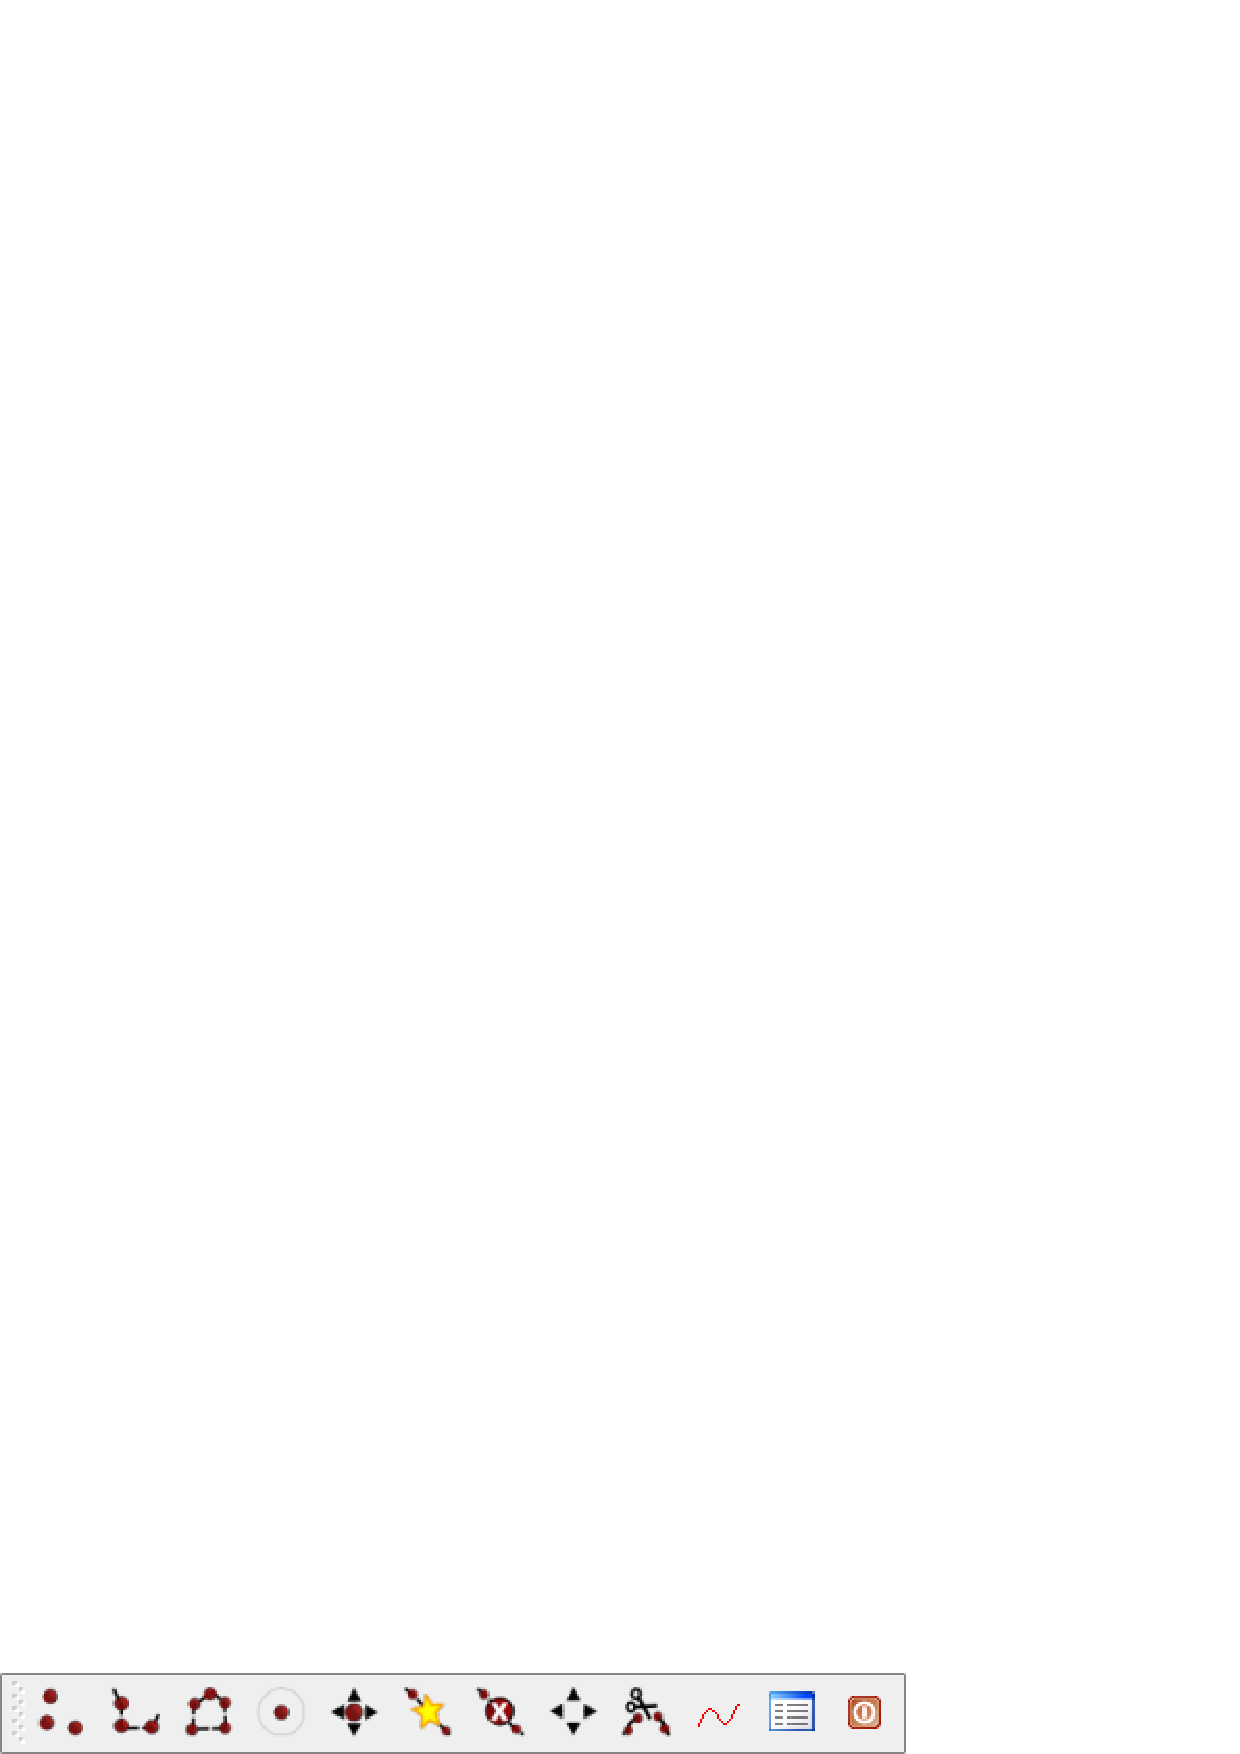
\includegraphics[clip=true,width=12cm]{grass_digitizing_toolbar}
\end{center}  
\end{figure}

\begin{table}[h]\index{GRASS!digitizing tools}
\centering
\caption{GRASS Digitizing Tools}\label{tab:grass_tools}\medskip
 \begin{tabular}{|l|l|p{5in}|}
 \hline \textbf{Icon} & \textbf{Tool} & \textbf{Purpose} \\
\hline 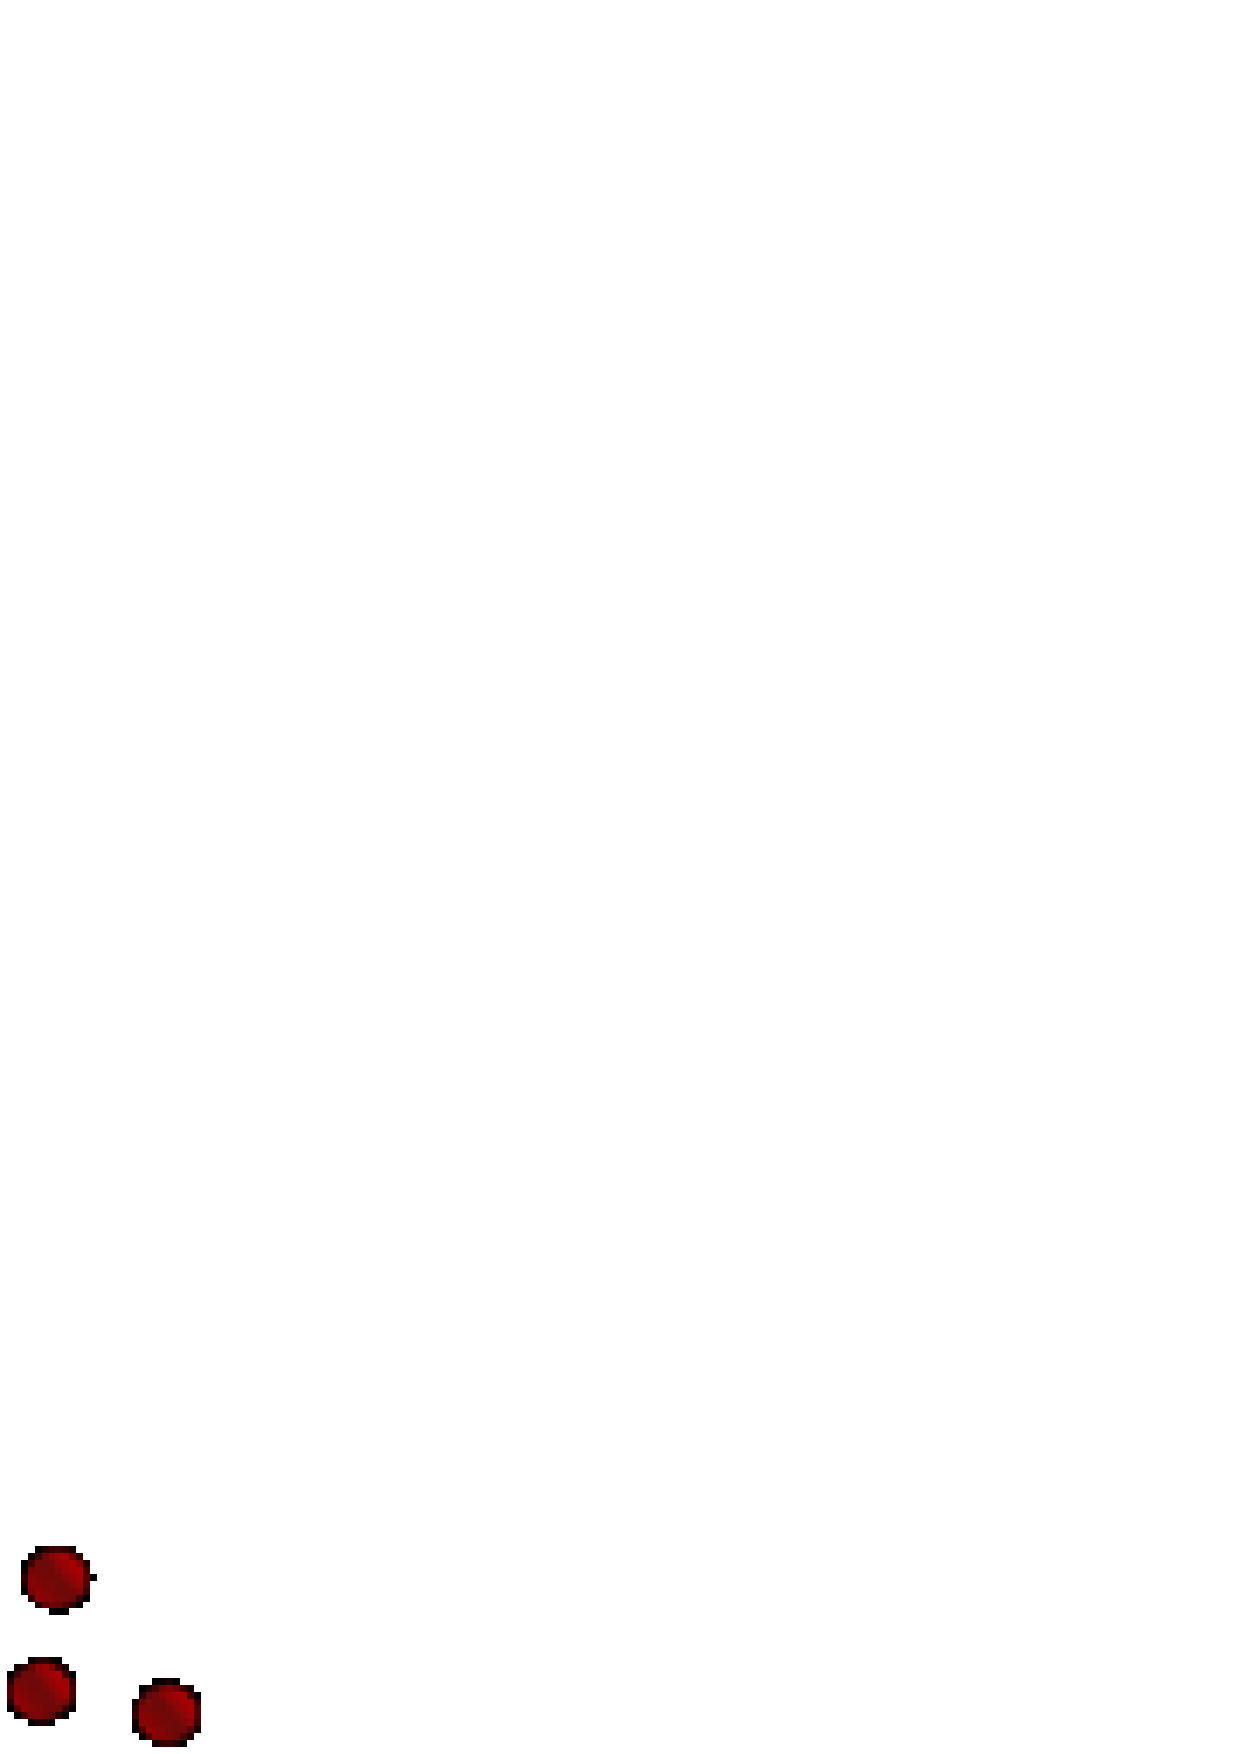
\includegraphics[width=0.7cm]{grass_new_point} & New Point & Digitize
new point \\
\hline 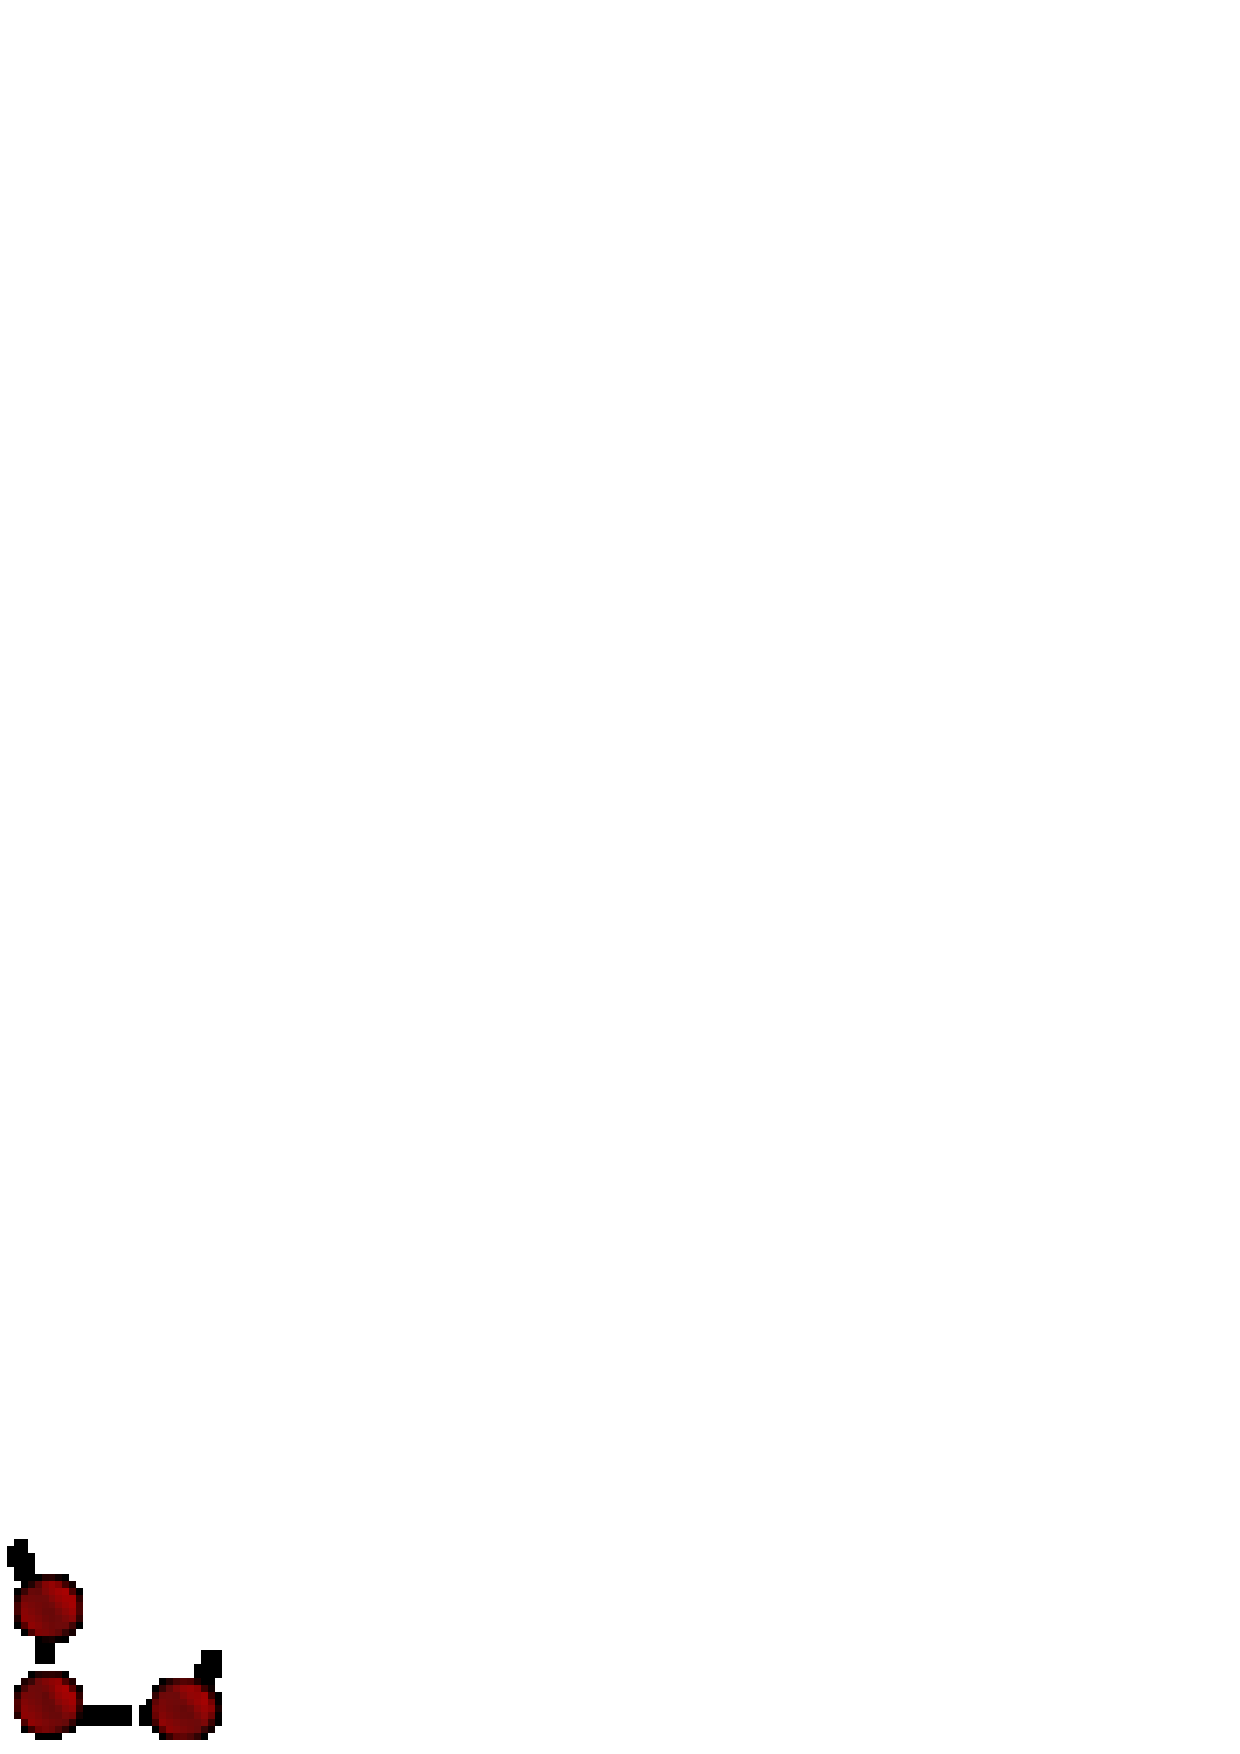
\includegraphics[width=0.7cm]{grass_new_line} & New Line & Digitize
new line (finish by selecting new tool) \\
\hline 
\includegraphics[width=0.7cm]{grass_new_boundary} & New Boundary &
Digitize new boundary (finish by selecting new tool)\\
\hline 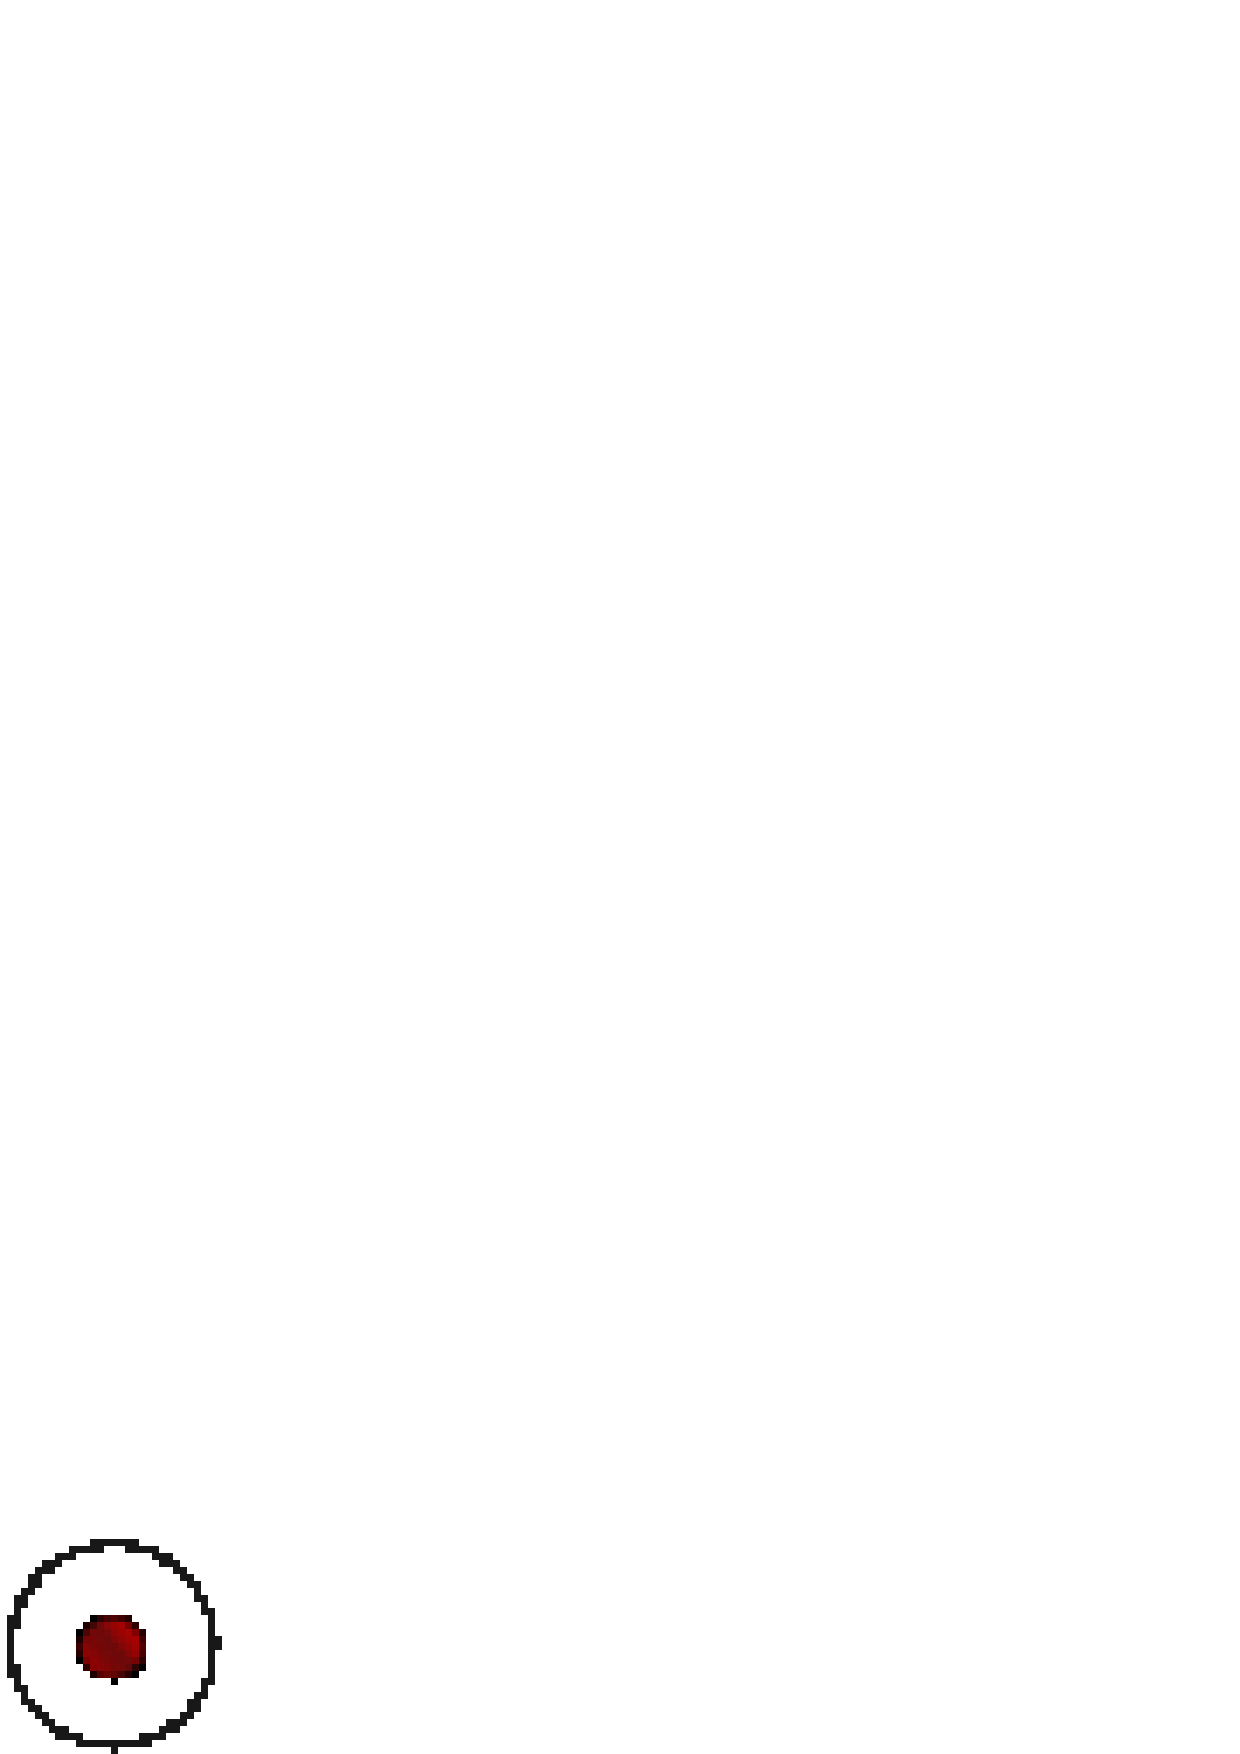
\includegraphics[width=0.7cm]{grass_new_centroid} & New Centroid &
Digitize new centroid (label existing area)\\
\hline 
\includegraphics[width=0.7cm]{grass_move_vertex} & Move vertex & Move
one vertex of existing line or boundary and identify new position\\
\hline 
\includegraphics[width=0.7cm]{grass_add_vertex} & Add vertex & Add a
new vertex to existing line\\
\hline 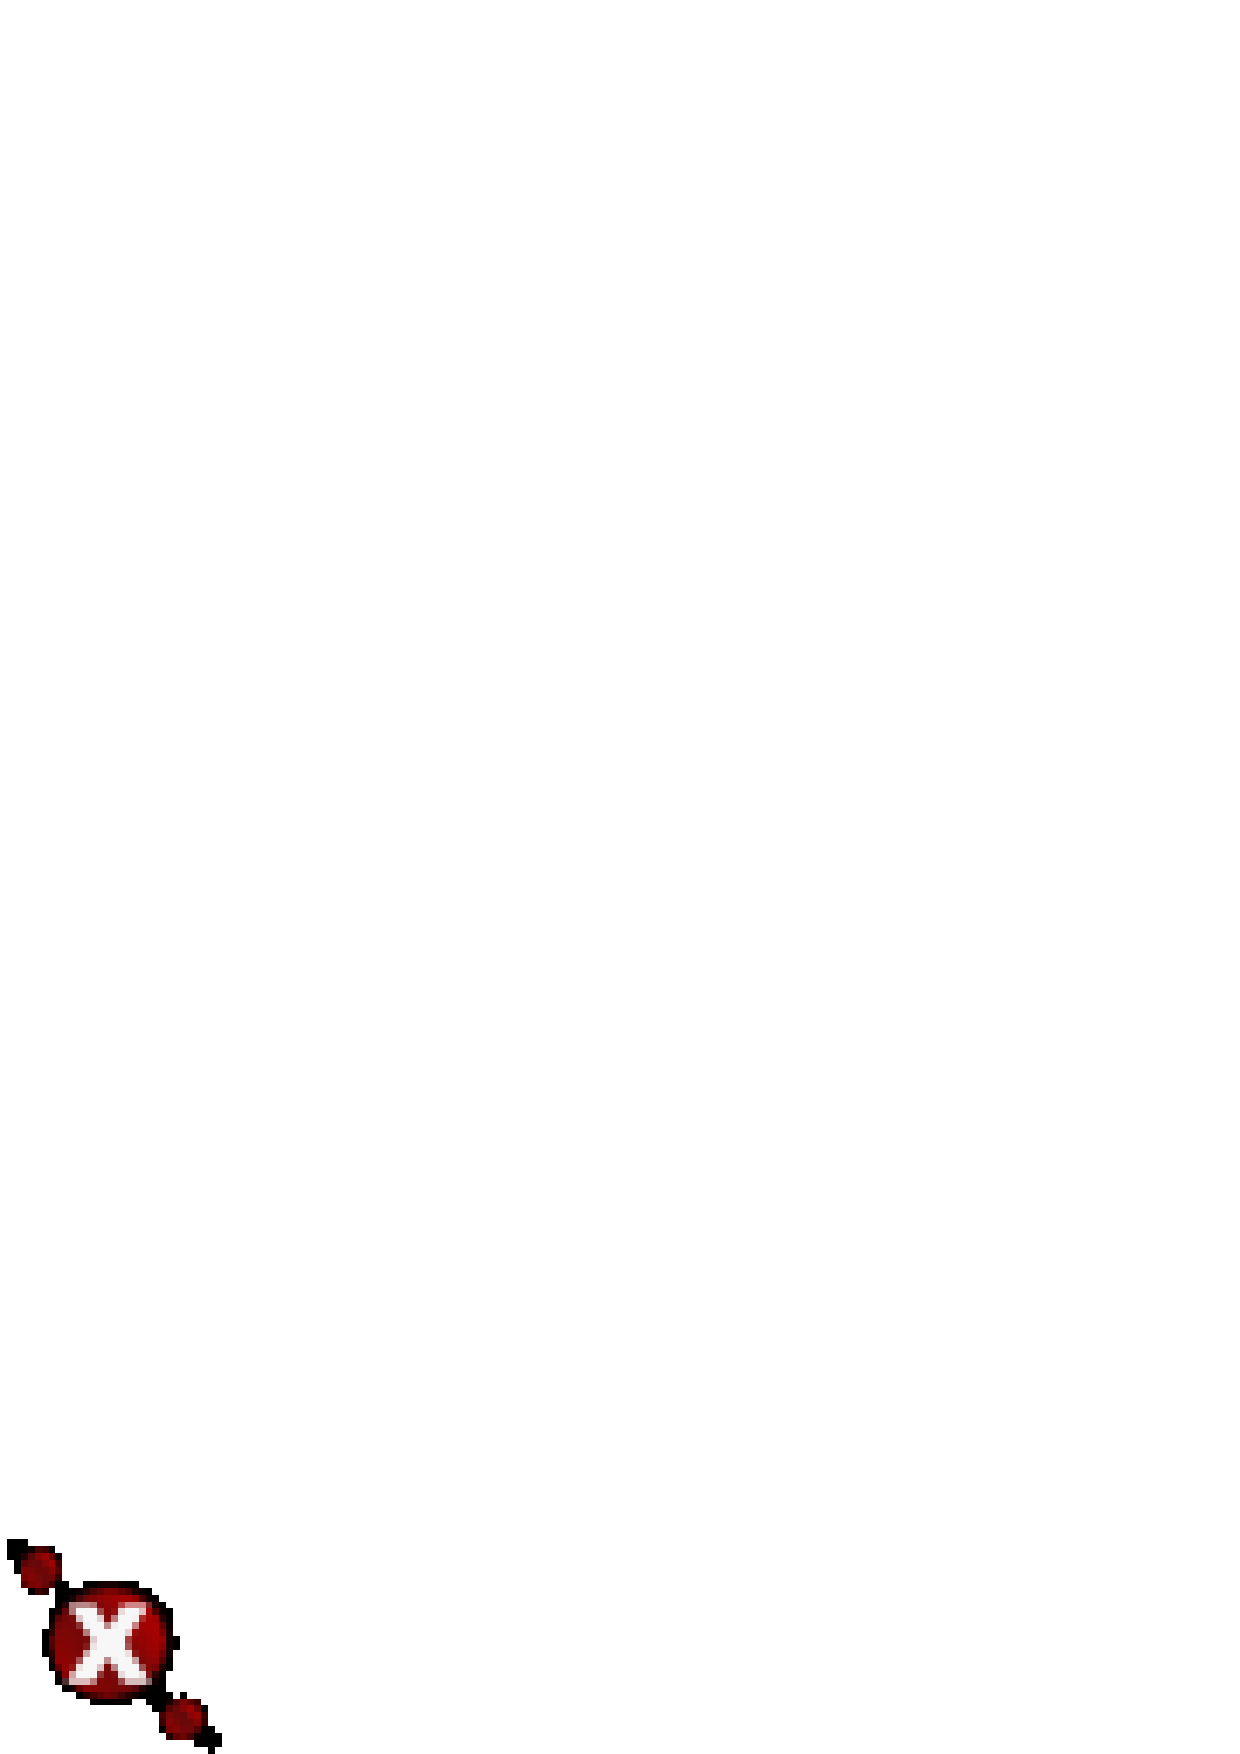
\includegraphics[width=0.7cm]{grass_delete_vertex} & Delete vertex &
Delete vertex from existing line (confirm selected vertex by another click)\\
\hline 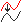
\includegraphics[width=0.7cm]{grass_move_line} & Move element & Move
selected boundary, line, point or centroid and click on new position\\
\hline 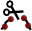
\includegraphics[width=0.7cm]{grass_split_line} & Split line & Split
an existing line to 2 parts\\
\hline 
\includegraphics[width=0.7cm]{grass_delete_line} & Delete element &
Delete existing boundary, line, point or centroid (confirm selected element by
another click)\\
\hline 
\includegraphics[width=0.7cm]{grass_edit_attributes} & Edit attributes
& Edit attributes of selected element (note that one element can represent
more features, see above)\\
\hline 
\includegraphics[width=0.7cm]{grass_close_edit} & Close & Close
session and save current status (rebuilds topology afterwards)\\
\hline
\end{tabular}
\end{table}

\minisec{Category Tab}\index{GRASS!category settings}

The \tab{Category} tab allows you to define the way in which the category 
values will be assigned to a new geometry element.

\begin{figure}[h]
 \begin{center}
  \caption{GRASS Digitizing Category Tab \nixcaption}\label{fig:grass_digitizing_category}
  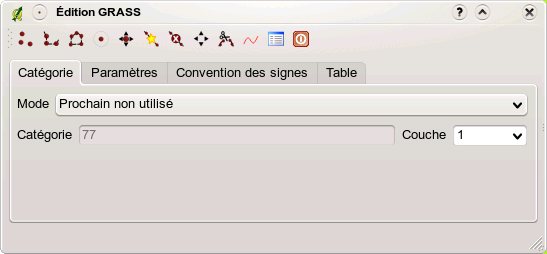
\includegraphics[clip=true,width=10cm]{grass_digitizing_category}
 \end{center}
\end{figure}

\begin{itemize}
\item \textbf{Mode}: what category value shall be applied to new geometry 
elements.
\begin{itemize}
\item Next not used - apply next not yet used category value to geometry
element.
\item Manual entry - manually define the category value for the geometry
element in the 'Category'-entry field.
\item No category - Do not apply a category value to the geometry element.
This is e.g. used for area boundaries, because the category values are
connected via the centroid.
\end{itemize}
\item \textbf{Category} - A number (ID) is attached to each digitized geometry
element. It is used to connect each geometry element with its attributes.
\item \textbf{Field (layer)} - Each geometry element can be connected with
several attribute tables using different GRASS geometry layers. Default layer
number is 1. 
\end{itemize}

\begin{Tip}\caption{\textsc{Creating an additional GRASS 'layer' with QGIS}}
\qgistip{If you would like to add more layers to your dataset, just add a new
number in the 'Field (layer)' entry box and press return. In the Table tab
you can create your new table connected to your new layer.
}
\end{Tip}

\minisec{Settings Tab}\label{label_settingtab}\index{GRASS!snapping
tolerance}

The \tab{Settings} tab allows you to set the snapping in screen pixels. The
threshold defines at what distance new points or line ends are snapped to
existing nodes. This helps to prevent gaps or dangles between boundaries. The
default is set to 10 pixels.

\begin{figure}[h]
 \begin{center}
 \caption{GRASS Digitizing Settings Tab \nixcaption}\label{fig:grass_digitizing_settings}
 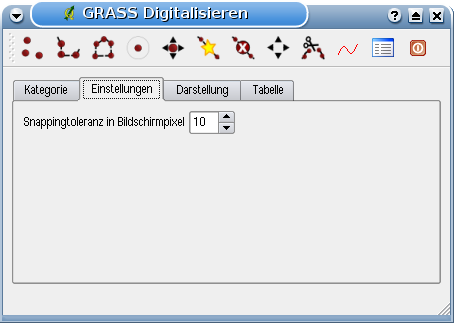
\includegraphics[clip=true,width=8cm]{grass_digitizing_settings}
 \end{center}
\end{figure}

\minisec{Symbology Tab}\index{GRASS!symbology settings}

The \tab{Symbology} tab allows you to view and set symbology and color
settings for various geometry types and their topological status (e.g. closed
/ opened boundary).

\begin{figure}[h]
 \begin{center}
 \caption{GRASS Digitizing Symbolog Tab \nixcaption}\label{fig:grass_digitizing_symbology}
 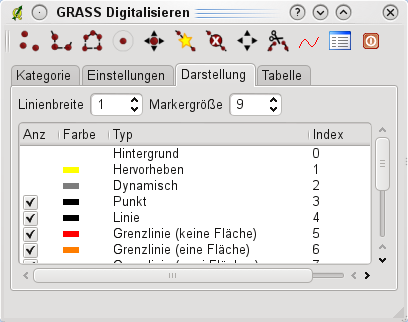
\includegraphics[clip=true,width=8cm]{grass_digitizing_symbology}
 \end{center}
\end{figure}

\minisec{Table Tab} \index{GRASS!table editing}

The \tab{Table} tab provides information about the database table for
a given 'layer'. Here you can add new columns to an existing attribute table,
or create a new database table for a new GRASS vector layer (see Section 
\ref{sec:creating_new_grass_vectors}).

\begin{figure}[h]
 \begin{center}
 \caption{GRASS Digitizing Table Tab \nixcaption}\label{fig:grass_digitizing_table}
 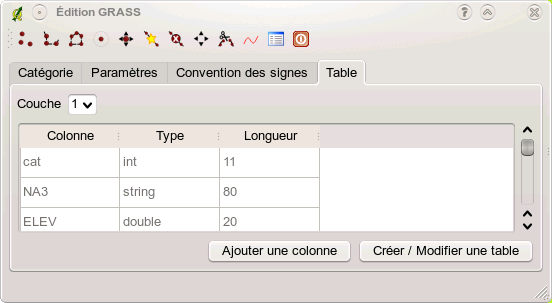
\includegraphics[clip=true,width=10cm]{grass_digitizing_table}
 \end{center}
\end{figure}

\begin{Tip}\caption{\textsc{GRASS Edit Permissions}}\index{GRASS!edit
permissions}
\qgistip{You must be the owner of the GRASS \filename{MAPSET} you want to 
edit. It is impossible to edit data layers in a \filename{MAPSET} that is not 
yours, even if you have write permissions.
}
\end{Tip} 

\subsection{The GRASS region tool}\label{sec:grass_region}\index{GRASS!region}

The region definition (setting a spatial working window) in GRASS is important 
for working with raster layers. Vector analysis is per default not limited
to any defined region definitions. All newly-created rasters will have the
spatial extension and resolution of the currently defined GRASS region,
regardless of their original extension and resolution. The current GRASS
region is stored in the \filename{\$LOCATION/\$MAPSET/WIND} file, and it 
defines north, south, east and west bounds, number of columns and rows, 
horizontal and vertical spatial resolution.

It is possible to switch on/off the visualization of the GRASS region in the
QGIS canvas using the \toolbtntwo{grass_region}{Visualizza GRASS regione attuale}
button. \index{GRASS!region!display}.

With the \toolbtntwo{grass_region_edit}{Modifica region GRASS attuale} icon you 
can open a dialog to change the current region and the symbology of the GRASS 
region rectangle in the QGIS canvas. Type in the new region bounds and 
resolution and click \button{OK}. It also allows to select a new region 
interactively with your mouse on the QGIS canvas. Therefore click with the 
left mouse button in the QGIS canvas, open a rectangle, close it using the 
left mouse button again and click \button{OK}.\index{GRASS!region!editing}
The GRASS module \filename{g.region} provide a lot more parameters to define 
an appropriate region extend and resolution for your raster analysis. You can 
use these parameters with the GRASS Toolbox, described in Section 
\ref{subsec:grass_toolbox}.

\subsection{The GRASS toolbox}\label{subsec:grass_toolbox}\index{GRASS!toolbox}

The \toolbtntwo{grass_tools}{Open GRASS Tools} box provides GRASS module 
functionalities to work with data inside a selected GRASS \filename{LOCATION} 
and \filename{MAPSET}. To use the GRASS toolbox you need to open a 
\filename{LOCATION} and \filename{MAPSET} where you have write-permission 
(usually granted, if you created the \filename{MAPSET}). This is necessary, 
because new raster or vector layers created during analysis need to be written 
to the currently selected \filename{LOCATION} and \filename{MAPSET}.

\subsubsection{Working with GRASS modules}\index{GRASS!toolbox}

\begin{figure}[h]
\centering
\caption{GRASS Toolbox and searchable Modules List \nixcaption}\label{fig:grass_modules}
   \subfigure[Modules Tree] {\label{subfig:grass_module_tree}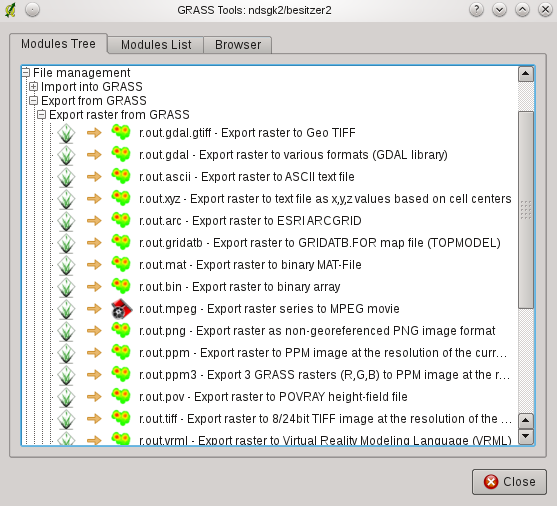
\includegraphics[clip=true, width=0.4\textwidth]{grass_toolbox_moduletree}}\goodgap
   \subfigure[Searchable Modules List] {\label{subfig:grass_module_list}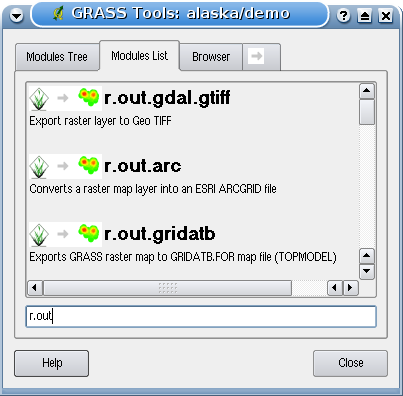
\includegraphics[clip=true, width=0.4\textwidth]{grass_toolbox_modulelist}}
\end{figure}

The GRASS Shell inside the GRASS Toolbox provides access to almost all (more 
than 300) GRASS modules in command line modus. To offer a more user
friendly working environment, about 200 of the available GRASS modules and 
functionalities are also provided by graphical dialogs. These dialogs are 
grouped in thematic blocks, but are searchable as well. You find a complete 
list of GRASS modules available in QGIS version \CURRENT
in appendix \ref{appdx_grass_toolbox_modules}. It is also possible to 
customize the GRASS Toolbox content. It is described in Section 
\ref{sec:toolbox-customizing}.

As shown in Figure \ref{fig:grass_modules}, you can look for the appropriate 
GRASS module using the thematically grouped \tab{Modules Tree} or the 
searchable \tab{Modules List} tab. 

Clicking on a grapical module icon a new tab will be added to the toolbox 
dialog providing three new sub-tabs \tab{Options}, \tab{Output} and 
\tab{Manual}. In Figure \ref{fig:grass_module_dialog} you see an example 
for the GRASS module \filename{v.buffer}.

\begin{figure}[h]
\centering
\caption{GRASS Toolbox Module Dialogs \nixcaption}\label{fig:grass_module_dialog}
   \subfigure[Module Options] {\label{subfig:grass_module_option}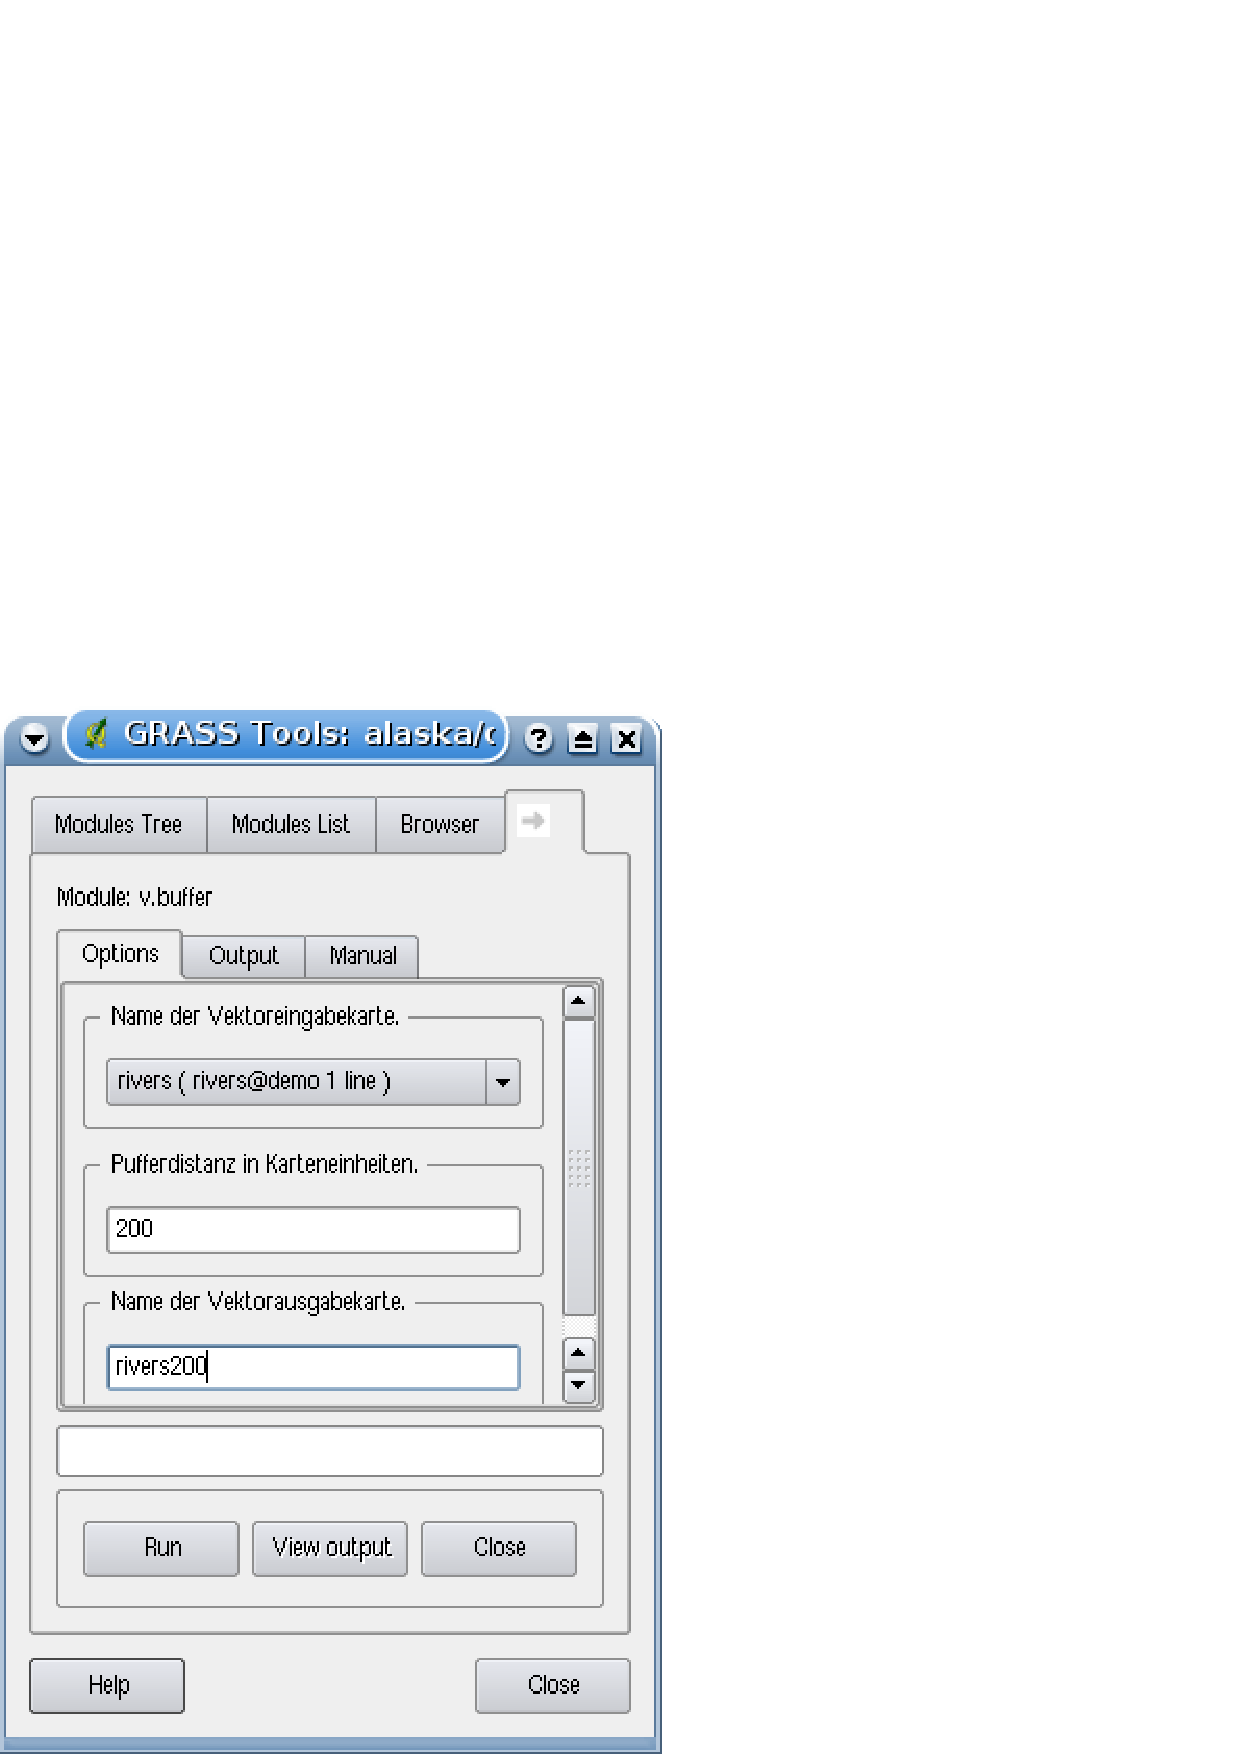
\includegraphics[clip=true, width=0.3\textwidth]{grass_module_option}}\goodgap
   \subfigure[Modules Output] {\label{subfig:grass_module_output}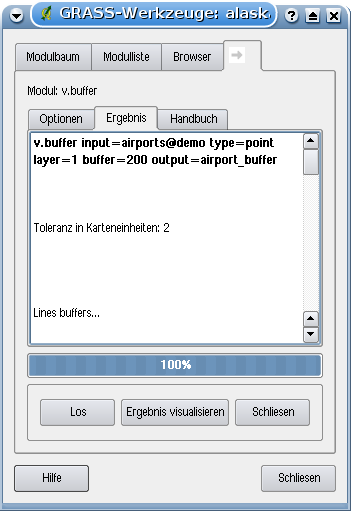
\includegraphics[clip=true, width=0.3\textwidth]{grass_module_output}}\goodgap
   \subfigure[Module Manual] {\label{subfig:grass_module_manual}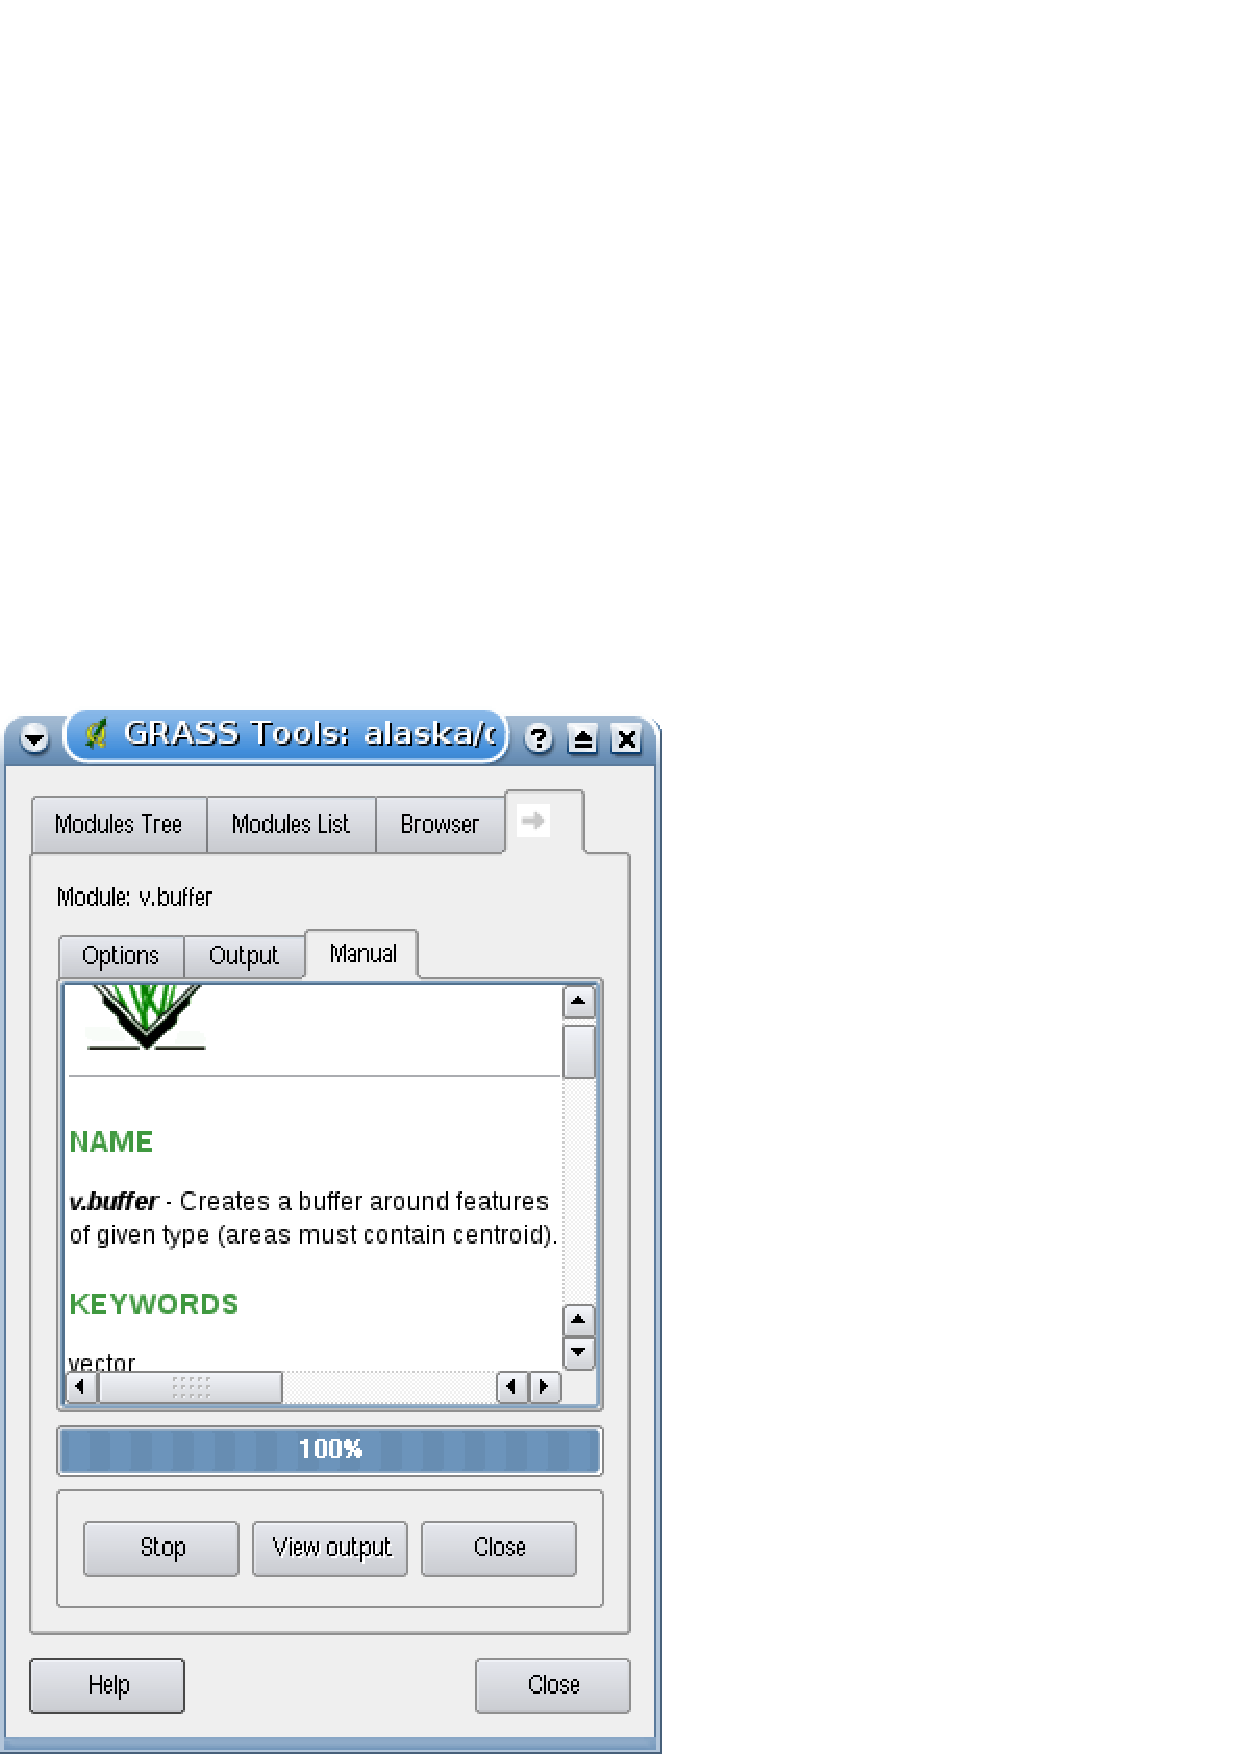
\includegraphics[clip=true, width=0.3\textwidth]{grass_module_manual}}
\end{figure}

\minisec{Options}

The \tab{Options} tab provides a simplified module dialog where you can 
usually select a raster or vector layer visualized in the QGIS canvas and 
enter further module specific parameters to run the module. The provided 
module parameters are often not complete to keep the dialog clear. If you want 
to use further module parameters and flags, you need to start the GRASS Shell 
and run the module in the command line.

\minisec{Output}

The \tab{Output} tab provides information about the output status of the 
module. When you click the \button{Run} button, the module switches to the 
\tab{Output} tab and you see information about the analysis process. If all 
works well, you will finally see a \usertext{Successfully finished} message.

\minisec{Manual}

The \tab{Manual} tab shows the HTML help page of the GRASS module. You can 
use it to check further module parameters and flags or to get a deeper 
knowledge about the purpose of the module. At the end of each module 
manual page you see further links to the \filename{Main Help index}, the 
\filename{Thematic index} and the \filename{Full index}. These links provide 
the same information as if you use the module \filename{g.manual} 

\begin{Tip}\caption{\textsc{Display results immediately}}\index{GRASS!display results}
\qgistip{If you want to display your calculation results immediately in your 
map canvas, you can use the 'View Output' button at the bottom of the 
module tab.
}
\end{Tip} 

\subsubsection{Working with the GRASS LOCATION browser} \index{GRASS!toolbox!Browser}

Another useful feature inside the GRASS Toolbox is the GRASS 
\filename{LOCATION} browser. In Figure~\ref{fig:grass_mapset_browser} you 
can see the current working \filename{LOCATION} with its \filename{MAPSETs}.

In the left browser windows you can browse through all \filename{MAPSETs} 
inside the current \filename{LOCATION}. The right browser window shows some 
meta information for selected raster or vector layers, e.g. resolution, 
bounding box, data source, connected attribute table for vector data and a 
command history.

\begin{figure}[h]
 \begin{center}
 \caption{GRASS LOCATION browser \nixcaption}\label{fig:grass_mapset_browser}
 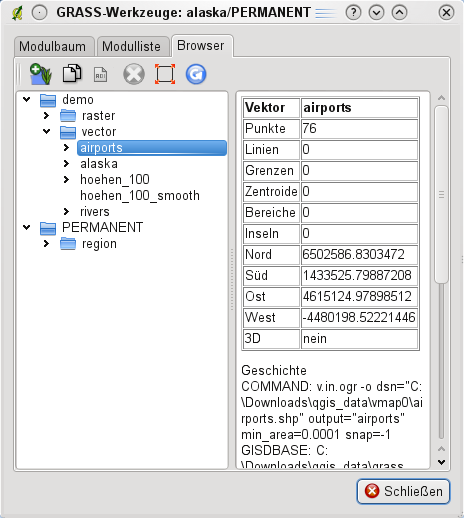
\includegraphics[clip=true,width=10cm]{grass_mapset_browser}
 \end{center}
\end{figure}

The toolbar inside the \tab{Browser} tab offers following tools to manage 
the selected \filename{LOCATION}:

\begin{itemize}
\item \toolboxtwo{grass_add_map}{Add selected map to canvas}
\item \toolboxtwo{grass_copy_map}{Copy selected map}
\item \toolboxtwo{grass_rename_map}{Rename selected map}
\item \toolboxtwo{grass_delete_map}{Delete selected map}
\item \toolboxtwo{grass_set_region}{Set current region to selected map}
\item \toolboxtwo{grass_refresh}{Refresh browser window}
\end{itemize}

The \toolboxtwo{grass_rename_map}{Rename selected map} and 
\toolboxtwo{grass_delete_map}{Delete selected map} only work with maps inside 
your currently selected \filename{MAPSET}. All other tools also work with 
raster and vector layers in another \filename{MAPSET}.

\subsubsection{Customizing the GRASS Toolbox} \index{GRASS!toolbox!customize}
\label{sec:toolbox-customizing}

Nearly all GRASS modules can be added to the GRASS toolbox. A XML 
interface is provided to parse the pretty simple XML files which configures 
the modules appearance and parameters inside the toolbox.

A sample XML file for generating the module \usertext{v.buffer} (v.buffer.qgm) 
looks like this:
\begin{verbatim}
<?xml version="1.0" encoding="UTF-8"?>
<!DOCTYPE qgisgrassmodule SYSTEM "http://mrcc.com/qgisgrassmodule.dtd">

<qgisgrassmodule label="Vector buffer" module="v.buffer">
        <option key="input" typeoption="type" layeroption="layer" />
        <option key="buffer"/>
        <option key="output" />
</qgisgrassmodule>
\end{verbatim}

The parser reads this definition and creates a new tab inside the toolbox 
when you select the module. A more detailed description for adding new 
modules, changing the modules group, etc. can be found on the QGIS wiki at \\
\url{http://wiki.qgis.org/qgiswiki/Adding\_New\_Tools\_to\_the\_GRASS\_Toolbox}.

